\documentclass[10pt,letterpaper]{article}
\usepackage[margin=0.8in]{geometry}
\usepackage{booktabs}
\usepackage{setspace}
\usepackage{tabularx}
\usepackage{array}
\usepackage{hyperref}
\usepackage{enumitem}
\usepackage{titlesec}
\usepackage{parskip}
\usepackage{microtype}
\usepackage{xcolor}
\usepackage{float}
\usepackage{graphicx}
\usepackage{caption}
\usepackage{amsmath}
\usepackage{amssymb}
\usepackage{setspace}
\sloppy
\hbadness=10000
\vbadness=10000

\titlespacing*{\section}{0pt}{6pt}{2pt}
\titlespacing*{\subsection}{0pt}{4pt}{1pt}
\setlength{\parskip}{2pt}
\setlength{\parindent}{0pt}

\definecolor{headblue}{RGB}{31,56,100}
\definecolor{subblue}{RGB}{46,116,181}

\titleformat{\section}{\large\bfseries\color{headblue}}{}{0em}{}
\titleformat{\subsection}{\normalsize\bfseries\color{subblue}}{}{0em}{}

\title{\textbf{CPS572 Final Project: Multi-Task LLM Fine-Tuning}}
\author{Aaron Huberman \and Qavi Inan}
\date{}

\begin{document}
\maketitle
\vspace{-24pt}

% =============================================================================
\section{1. Methodology}
% =============================================================================

\subsection{1.1 Problem Setup and Approach}
\vspace{5pt}
This project fine-tunes \texttt{meta-llama/Llama-3.1-8B} via Low-Rank Adaptation (LoRA) 
to simultaneously improve IFEval (instruction following), GSM8K (mathematical reasoning), 
and HumanEval (code generation). We began with the smaller Llama-3.2-3B model trained on 
the three suggested datasets (GSM8K, Tulu-3, OpenCodeInstruct) to establish a working 
baseline, then scaled to 8B. From there we identified additional high-quality datasets, 
performed hyperparameter tuning, experimented with system prompts, and implemented GRPO 
training. Our best configuration was trained for 16,000 steps with checkpoints saved every 
1,000 steps; the checkpoint maximizing average score across all three tasks was selected 
for final submission.

\subsection{1.3 Dataset Composition}

The final model trained on the following 6 datasets:
\begin{table}[H]
\centering
\footnotesize
\begin{tabularx}{\textwidth}{llrX}
\toprule
\textbf{Dataset} & \textbf{Task} & \textbf{Size Used} & \textbf{Notes} \\
\midrule
openai/gsm8k (train split) & Math & 7,473 & Full train set; CoT prefix added \\
microsoft/orca-math-word-problems-200k & Math & 50,000 & GPT-4 generated diverse math problems \\
meta-math/MetaMathQA & Math & 50,000 & GSM8K/MATH rewrites via paraphrase and self-verify \\
allenai/tulu-3-sft-mixture & IF & 100,000 & General instruction following mixture \\
argilla/ifeval-like-data (filtered) & IF & 56,339 & All verified IFEval-constraint examples \\
nvidia/OpenCodeInstruct & Code & 100,000 & Quality filtered at $\geq 0.9$ test pass rate \\
\bottomrule
\end{tabularx}
\end{table}

The math pool (GSM8K + Orca-Math + MetaMathQA) totals approximately 107,000 examples. Each dataset was included for the following reasons. GSM8k was a suggested dataset and started as our core for math training. Orca-Math claims "This dataset has been designed to enhance the mathematical abilities of language models," after testing we found it effective.  MetaMathQA provides benefits via problem rewriting generating paraphrases, reverse questions, and self-verification variants of existing GSM8K and MATH problems, exposing the model to the same underlying reasoning challenges with varied phrasing. An important note about MetaMathQA it specifically lists that none of the augmented data is from the testing set of GSM8k.


The instruction following pool combines two complementary datasets. Tulu-3 was included as the baseline IF dataset since it was suggested. This was then augmented with Argilla ifeval like data. Through testing we saw that our model was specifically failing mechanical constraint following type questions such as "answer without using commas." Adding the Argilla dataset 
specifically targeting IFEval constraint types, helped with prompt adherence. These two datasets were found to be complementary: Tulu handles the easy IFEval constraints the model already partially knows (JSON format, response language, postscript), while Argilla specifically targets the hard mechanical constraints where we measured high failure rates.

Finally for code we only used  OpenCodeInstruct the suggested dataset. However, we filtered to examples with \texttt{average\_test\_score} $\geq 0.9$, meaning only code solutions that pass at least 9 of 10 unit tests are included. This quality filter rejects noisy or incorrect code examples that would degrade training signal.

Another note: the simple data filtering we performed was all done in the main body \texttt{train\_and\_publish} since it was relatively simple.

\subsection{1.4 Data Mixing and Hyperparameters}

Datasets were combined using weighted random sampling: math 2.0, IF (Tulu + Argilla) 
4.0, code 2.0. The higher IF weight reflects IFEval being our most challenging task. 
Hyperparameters were initially tuned on Llama-3.2-3B for iteration speed, then 
transferred directly to the 8B model without further adjustment. A full table of hyperparameter used are provided below

\subsection*{Full Hyperparameter Table}

\begin{table}[H]
\centering
\footnotesize
\begin{tabularx}{\textwidth}{llX}
\toprule
\textbf{Parameter} & \textbf{Final Value} & \textbf{Rationale} \\
\midrule
Learning rate & 5e-5 (initial), 3e-5 (continuation) & Reduced for continuation to avoid overshooting \\
Warmup steps & 200 (initial), 100 (continuation) & Linear warmup stabilizes early rank-128 updates \\
Weight decay & 0.01 & L2 regularization; reduces overfitting on large dataset \\
Gradient clip norm & 1.0 & Prevents destabilizing spikes from hard batches \\
Adam $\beta_1, \beta_2$ & 0.9, 0.95 & Standard values for LLM fine-tuning \\
Batch size & 4 & Tinker API constraint \\
Max sequence length & 1024 & Captures full chain-of-thought reasoning steps \\
LoRA rank & 128 & Multi-task adaptation capacity \\
\bottomrule
\end{tabularx}
\end{table}


\subsection{1.5 Training Procedure}
Early experiments used shorter runs of 500--2,000 steps on smaller models (Llama-3.2-3B 
and Llama-3.1-8B) to validate the pipeline and iterate on dataset selection and 
hyperparameters. Once the final configuration was established, we trained the 8B model 
to convergence over 16,000 total steps across two phases. Phase 1 ran for 8,000 steps 
from a freshly initialized LoRA adapter, with checkpoints saved every 1,000 steps. 
Phase 2 resumed from the step-8000 checkpoint with a slightly reduced learning rate 
(3e-5) and a fresh random seed to expose new example orderings. All intermediate 
checkpoints were evaluated on all three tasks, and the checkpoint maximizing average 
score across IFEval, GSM8K, and HumanEval was selected for final submission.


% =============================================================================
\section{2. Extensions}
% =============================================================================

\subsection{2.1 Targeted Data Selection for IFEval}

Our first extension was  data augmentation to improve IFEval performance. After 
noticing that IFEval scores plateaued despite increasing the Tulu-3 sample size, we 
investigated exactly what the model was getting wrong rather than simply adding more 
of the same data.

IFEval tests 22 distinct constraint types. We wrote a script to parse the detailed 
evaluation logs saved by Inspect AI and compute per-constraint pass and fail rates 
across all 541 test prompts. This revealed three clear failure clusters:

\begin{itemize}[noitemsep,topsep=2pt]
\item \textbf{Case constraints (95--100\% failure):} The model almost never obeys 
capitalization instructions such as ``write in all lowercase'' or ``capitalize every 
word'' --- \texttt{english\_lowercase} (100\%), \texttt{english\_capital} (92\%), 
\texttt{capital\_word\_frequency} (84\%)
\item \textbf{Length and count constraints (79--100\% failure):} The model does not 
count words, sentences, or paragraphs while generating --- 
\texttt{nth\_paragraph\_first\_word} (100\%), \texttt{number\_paragraphs} (93\%), 
\texttt{number\_words}/\texttt{number\_sentences} (79\%)
\item \textbf{Keyword constraints (79--84\% failure):} The model does not track 
required or forbidden words --- \texttt{forbidden\_words} (84\%), 
\texttt{keywords:frequency} (81\%), \texttt{keywords:existence} (79\%)
\end{itemize}

The root cause is that Tulu-3, while a strong general instruction-following dataset, 
contains no examples of these mechanical constraint types. Natural conversational 
responses are not written in all-lowercase or to exact word counts, so no amount of 
Tulu-3 data can teach the model these skills.

To address this, we identified \texttt{argilla/ifeval-like-data} (filtered subset): 
56,339 examples generated by Qwen2.5-72B-Instruct and programmatically verified 
against the IFEval constraint checker, covering all the high-failure constraint types 
we identified. Replacing Tulu-3 with this dataset in v4 produced an 18-point IFEval 
jump (41.9\% $\to$ 60.2\%)  the largest single improvement of the entire project 
confirming that the bottleneck was data relevance, not model capacity or training 
duration.

\subsection{2.2 Manual GRPO Implementation on an SFT-Only API}
The next major extension we implemented was GRPO training. We wrote code to generate 
$G$ candidate responses, score them with a reward function, and update the model toward 
higher-reward outputs. IFEval is a natural fit for this approach since the constraint 
checker provides a deterministic, programmatically computable reward.

Tinker does not natively support RL, so we implemented GRPO from Tinker primitives. 
The implementation required solving several engineering challenges not covered by 
Tinker's documentation. Each step: sample a prompt from argilla; generate $G{=}16$ 
responses via \texttt{create\_sampling\_client} at temperature 1.0; then score each 
with \texttt{instruction\_following\_eval}.

We used the following partial credit reward function, which awards fractional scores 
rather than binary pass/fail:
\[
r = \frac{1}{K} \sum_{k=1}^{K} \mathbf{1}[\text{constraint}_k \text{ satisfied}]
\]
Each constraint's parameters are passed individually to the checker to avoid key 
collisions when multiple constraints share parameter names. Group-relative advantages 
are then computed as $A_i = (r_i - \bar{r}) / (\sigma_r + \epsilon)$.

Responses with $A_i > 0$ become weighted training datums with token weights 
proportional to $A_i$; responses with $A_i \leq 0$ are discarded. Since Tinker exposes only SFT primitives, we omit the reference model KL penalty used in full GRPO, instead discarding negative-advantage responses rather than penalizing them. The gradient then updates with
\texttt{forward\_backward} + \texttt{optim\_step}.

% =============================================================================
\section{3. Results and Analysis}
% =============================================================================

\subsection{3.1 Experimental Progression}

In total we had 5 major iterations of our model, with minor tweaks between each major update. Below is the tracked progress of each model with key changes from the previous iteration as well as their performance on each task. Our final model (v5) without our GRPO extension ended up performing the best on average score.


\begin{table}[H]
\centering
\footnotesize
\begin{tabularx}{\textwidth}{lrrrl}
\toprule
\textbf{Version} & \textbf{IFEval} & \textbf{GSM8K} & \textbf{HumanEval} & \textbf{Key Change from Previous} \\
\midrule
Baseline (no FT) & 22.8\% & 9.7\% & 0.6\% & --- \\
v1 (3B, 500 steps) & 25.7\% & 26.0\% & 30.5\% & Real data, 3B model \\
v1 (8B, 500 steps) & 37.7\% & 51.3\% & 42.1\% & Scaled to 8B \\
v2 (8B, 1500 steps) & 41.9\% & 56.7\% & 46.3\% & Orca-Math, 50k Tulu, CoT \\
v3 (8B, 2000 steps) & 38.9\% & 58.9\% & 45.1\% & System prompting \\
v4 (8B, 2000 steps) & 60.2\% & 61.1\% & 48.2\% & Argilla replaces Tulu \\
v4b (8B, 2000 steps) & 61.5\% & 63.8\% & 45.7\% & Retrain with save\_state fix \\
v4b + GRPO & 61.3\% & 64.5\% & 46.3\% & 300-step GRPO on IFEval \\
v5 step 3000 & 62.5\% & 56.7\% & 42.7\% & Large dataset, early checkpoint \\
v5 step 5000 & 63.5\% & 63.7\% & 44.5\% & IFEval peak \\
v5 step 8000 & 63.0\% & 68.3\% & 45.7\% & GSM8K peak \\
v5b step 11000 & 64.2\% & 66.9\% & 43.3\% & Continuation, IFEval improves \\
v5b step 13000 & \textbf{65.2\%} & \textbf{68.5\%} & 46.3\% & \textbf{Best avg, submission checkpoint} \\
v5b step 16000 & 60.8\% & 68.5\% & \textbf{49.4\%} & HumanEval peak, IFEval regresses \\
\bottomrule
\end{tabularx}
\end{table}

We decided to train our model for 16,000 steps after seeing training loss continually and gradually going down. Since we didn't see any reversion after the initial 8,000 steps we loaded the save state and trained for another 16,000. Although the loss seems to continue to drop on average we started to see noticeable regression in the IFEval score between the submitted 13000 step and the final 16000 step checkpoint.

\begin{figure}[H]
\centering

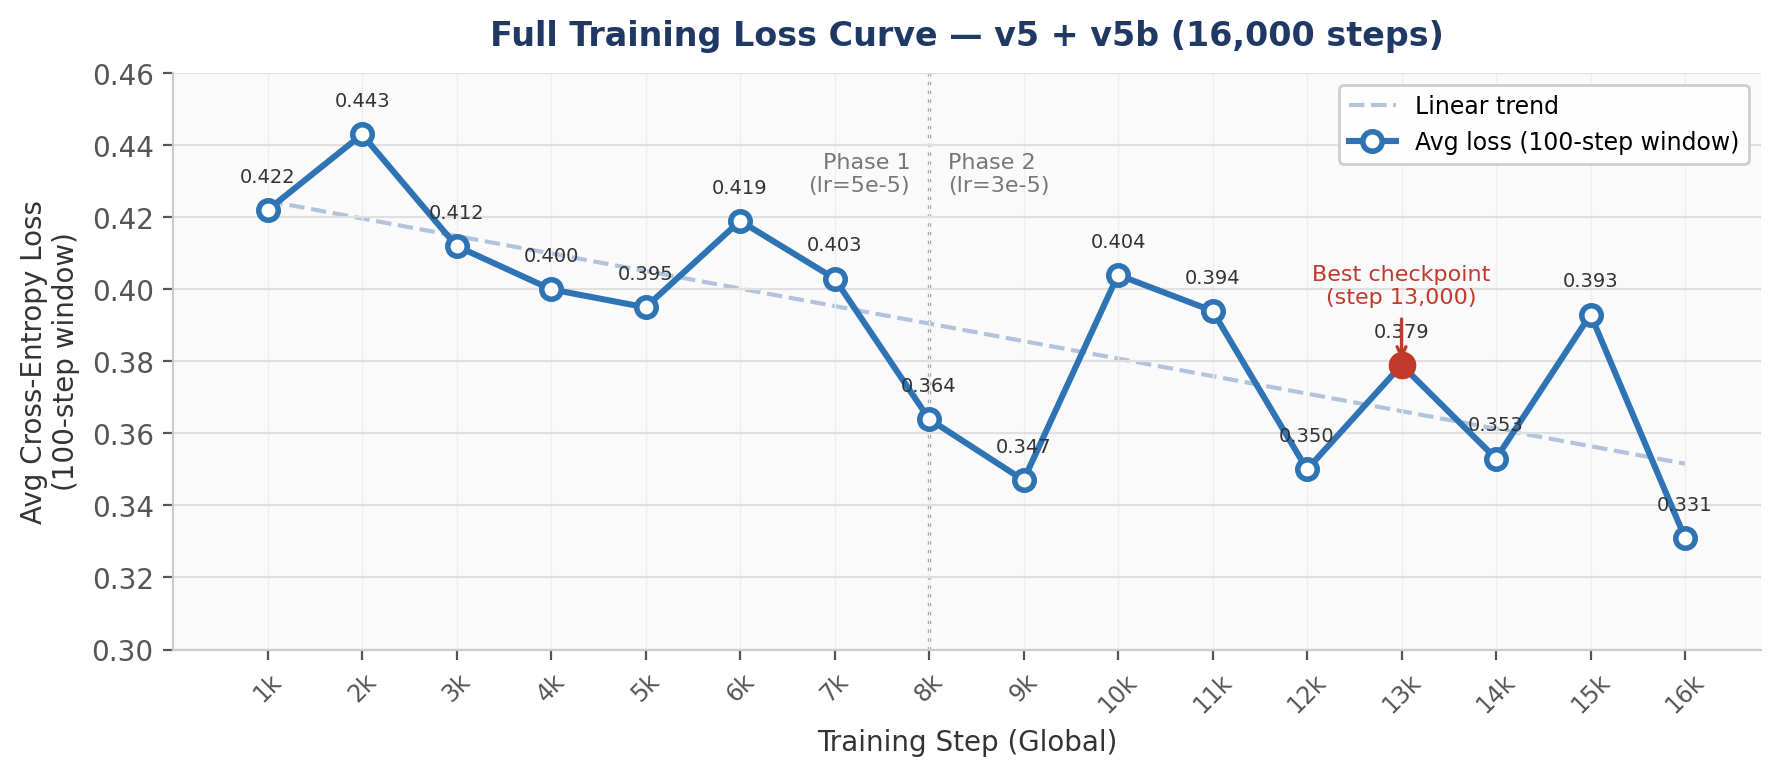
\includegraphics[width=\textwidth]{loss_curve_full.png}

\caption{Training loss over 16,000 steps showing continued convergence throughout the run.}
\end{figure}
\subsection{3.2 What Worked and Why}

\textbf{Scaling to 8B.} Moving from Llama-3.2-3B to Llama-3.1-8B produced the 
second-largest single improvement of the project (IFEval +12\%, GSM8K +25.3\%, 
HumanEval +11.6\%). Larger models have more capacity to store task-specific patterns 
and more robust representations from pretraining that fine-tuning can unlock. One 
important finding was that 3B and 8B results are not reliable predictors of each 
other: the 3B model excelled on HumanEval early but struggled on GSM8K, while 8B 
showed the opposite pattern. This led us to work exclusively with 8B for all 
subsequent experiments.

\textbf{Argilla dataset selection.} Replacing Tulu-3 with Argilla in v4 produced an 
18-point IFEval improvement, the largest single gain of the project. IFEval's hardest 
constraint types (lowercase, word count, forbidden words) require the model to monitor 
its own output during generation, a skill absent from natural instruction-following 
data. Argilla provides verified demonstrations of exactly these constraint types with 
no degradation on GSM8K or HumanEval.

\textbf{Multi-source math ensembling with CoT.} Combining GSM8K, Orca-Math, and 
MetaMathQA with chain-of-thought prefixes improved GSM8K from 51.3\% (v1) to 68.5\% 
(v5b step 13,000). CoT prefixes teach the model to decompose problems before 
answering. Since GSM8K scoring extracts the final number via regex, verbose 
intermediate reasoning does not penalize the score.

\textbf{Extended training to 16,000 steps.} After observing that training loss 
continued declining without signs of convergence at 8,000 steps, we resumed from the 
saved checkpoint for an additional 8,000 steps. At batch size 4 and 2,000 steps only 
about 2\% of the 363k-example dataset is seen per run, which is far too little for 
convergence. Extending to 16,000 steps improved GSM8K to 68.5\% and HumanEval to a 
peak of 49.4\%. However evaluation scores told a more nuanced story than the loss 
curve: IFEval peaked at step 13,000 (65.2\%) and regressed by step 16,000 (60.8\%), 
suggesting the model began overfitting to math and code at the expense of instruction 
following in the later stages. This highlights the importance of evaluating 
intermediate checkpoints rather than defaulting to the final one.

\textbf{Optimizer improvements.} Weight decay (0.01) and gradient clipping (norm 1.0) 
added in v3 stabilized training and smoothed loss curves in subsequent runs. Their 
absence in v1 and v2 likely contributed to the noisy loss behavior observed in those 
early experiments.

\textbf{Early stopping trade-offs.} No single checkpoint dominates all three tasks 
simultaneously. IFEval peaked at step 13,000 (65.2\%) while GSM8K and HumanEval 
continued improving through step 16,000. We selected step 13,000 as our submission 
checkpoint since it maximizes average score across all three tasks. Simply taking the 
final checkpoint would have cost nearly 5 points on IFEval.

\subsection{3.3 Negative Results and Failed Experiments}

\textbf{System prompt on Tulu data} We prepended a constraint-awareness 
system prompt to all 80,000 Tulu examples, hypothesizing it would activate 
constraint-following behavior. IFEval instead regressed from 41.9\% to 38.9\%. 
Post-hoc constraint analysis confirmed the system prompt worsened every constraint 
category. The most likely cause is that the model learned to prepend a 
constraint-checking preamble, causing failures on prompt-level strict scoring since 
compliance is required from the first token. Training Tulu examples with no explicit 
constraints under a constraint-checking system prompt also created incoherent training 
signal.



\textbf{Tulu-3 scaling} Increasing Tulu from 50k to 80k with 
higher IF weight did not improve IFEval. Generic instruction following data has a 
ceiling for mechanical constraint types. The model learns to follow natural language 
instructions but Tulu does not teach word counting or comma avoidance, which require 
fundamentally different training signal. This motivated the switch to Argilla.

\textbf{GRPO reward sparsity.} GRPO produced modest gains (GSM8K +0.7\%, HumanEval 
+0.6\%) but did not improve IFEval despite being specifically targeted at it. At 
60\%+ accuracy, most prompts fall into degenerate cases: easy prompts where all 
$G{=}16$ samples score 1.0, or hard prompts where all score 0.0. Both produce zero 
variance and no gradient signal. A denser reward function or targeted selection of 
high-failure prompts would be needed for GRPO to be effective at this performance 
level.



\vfill

\newpage

\subsection*{4. LLM Usage}

Claude (Anthropic, \texttt{claude-sonnet-4-6}) was used throughout this project. All usage is disclosed below.

\textbf{Code writing} Claude helped write code for this project, used most extensively in the implementation of \texttt{evaluation/grpo\_train.py}. Other than this, Claude was mainly used to debug Tinker API errors throughout, including identifying correct method signatures (\texttt{build\_generation\_prompt}, \texttt{save\_state}, \texttt{SampledSequence.tokens}, \texttt{create\_training\_client\_from\_state}), resolving import errors, and fixing Windows-specific issues (SSH key setup, PowerShell venv activation, HuggingFace Hub symlink warnings).

\textbf{Experimental design} Claude was periodically queried for potential ideas and next steps for the project.

\textbf{Analysis and interpretation} This is where Claude was most heavily leveraged, after each iteration of the model, outputs were given to Claude. Claude was then asked at the time of report writing to aggregate all scores by model version and document which model changes related to which improvements.

\textbf{Report writing.} Claude was used to set up an outline. The majority of the writing was done by us. Occasionally Claude was used to spell and grammar check writing. 
\subsection*{5. Tinker Platform Feedback}

\textbf{What was the hardest part?} The biggest source of friction was the gap between 
Tinker's SFT-oriented API and the more advanced training methods the project 
documentation explicitly encourages. Implementing GRPO required significant exploratory 
debugging. We had to discover through trial and error that \texttt{save\_state} rather 
than \texttt{save\_weights} is the correct method for a resumable checkpoint, that 
sampler weight paths and training state paths use different formats and cannot be used 
interchangeably, and that \texttt{create\_training\_client\_from\_state} rejects sampler 
paths with an opaque 400 error. A simple taxonomy of checkpoint path formats in the 
documentation would have saved several hours. Windows compatibility was a secondary 
issue since the project materials appear to assume a Unix environment, and several setup 
steps including SSH key configuration and HuggingFace Hub symlink behavior required 
workarounds not covered anywhere.

\textbf{Did you use the tinker-cookbook?} Yes, extensively. The cookbook was 
indispensable for conversation rendering, tokenization, and training datum construction. 
These abstractions work well and significantly reduce boilerplate. What was missing was 
documentation of \texttt{build\_generation\_prompt}'s return type since it returns a 
\texttt{ModelInput} object directly rather than a token list, which is non-obvious and 
caused our GRPO sampling to fail initially. Examples of advanced workflows such as 
checkpoint resumption and running a training client alongside a sampling client 
simultaneously would also have been helpful. We ended up using \texttt{dir()} and 
\texttt{inspect.signature()} to discover available methods, which works but should not 
be necessary.

\textbf{What one thing would make Tinker significantly better?} Native GRPO or PPO 
support. The project documentation lists reinforcement learning as an encouraged 
extension, and Tinker already has all the necessary primitives. However, combining them 
into a correct RL loop requires substantial undocumented engineering, and without a 
reference model for computing KL penalties our implementation is a simplified 
approximation. A \texttt{create\_grpo\_training\_client} analogous to 
\texttt{create\_lora\_training\_client} that handles sampling, advantage computation, 
and reference model management internally would dramatically lower the barrier and 
produce more principled experiments.

\textbf{Would you use Tinker again?} Yes. The ability to train an 8B model through a 
simple Python API without managing any GPU infrastructure was genuinely valuable for an 
academic project where the goal is experimentation rather than infrastructure 
engineering. Training for 8,000 steps with checkpointing completed reliably overnight 
with no configuration issues. The platform is clearly well-suited to the SFT use case 
it is designed for, and with better documentation and RL support it would be compelling 
for more advanced research workflows as well.

\end{document}
